\documentclass[10pt]{beamer}

%%%
% PREAMBLE FOR THIS DOC 
%%%
%https://tex.stackexchange.com/questions/68821/is-it-possible-to-create-a-latex-preamble-header
\usepackage{/Users/miw267/Repos/csci246_spring2025/slides/preambles/beamer_preamble_for_CSCI246}



%%% TRY TO RESHOW TOC AT EACH SECTION START (with current section highlighted)
% Reference: https://tex.stackexchange.com/questions/280436/how-to-highlight-a-specific-section-in-beamer-toc
\newcommand\tocforsect[2]{%
  \begingroup
  \edef\safesection{\thesection}
  \setcounter{section}{#1}
  \tableofcontents[#2,currentsection]
  \setcounter{section}{\safesection}
  \endgroup
}


%%%% HERES HOW TO DO IT CORRECTLY
% FIRST IN .STY FILE, DO
%\usetheme[sectionpage=none]{metropolis}
% THEN AT EACH SECTION DO
%\begin{frame}{Outline}
%  \tableofcontents[currentsection]	
%\end{frame}



%\setbeamertemplate{navigation symbols}{}
%\setbeamertemplate{footline}[frame number]{}


%%%
% DOCUMENT
%%%

\begin{document}

%\maketitle

%% Title page frame
%\begin{frame}
%    \titlepage 
%\end{frame}





\title{02/10/2025: Sets}
\author{CSCI 246: Discrete Structures}
\date{Textbook reference: Sec. 10, Scheinerman}

\begin{frame}
    \titlepage 
\end{frame}


\begin{frame}
\footnotesize 
\begin{mygreenbox}[title=Graded Quiz Pickup]
Quizzes are in the front of the room, grouped into four bins (A-G, H-L, M-R, S-Z) by last name. The quizzes are upside down with your last name on the back. Come find yours before, during, or after class.  Only turn the quiz over if it's yours.
\end{mygreenbox} 
\vfill 

%\begin{myredbox}[title=Announcements]
%
%\begin{itemize}
%\item Wednesday's reading quiz was graded out of 1 point.  45/60 students who took the quiz scored 100\%.
%\item Note: The reading quizzes are equally weighted.  The denominator is typically chosen for convenience.  
%\end{itemize}
%
%\end{myredbox}
%
%\vfill 


\begin{myyellowbox}[title=Today's Agenda]
\begin{itemize}
	\item Reading and problems quiz  (12 mins)
	\item Mini-lecture ($\approx$ 15 mins)
%	%
%	\begin{itemize}
%	\footnotesize 
%	\item Review induction 
%	\end{itemize}
%	%
	\item Group exercises ($\approx$ 20 mins)
\end{itemize}

\end{myyellowbox}
\vfill 

\end{frame}




\begin{frame}
\footnotesize 
%
%\alert{Reminder:} Please write your last name on the back of your page.
%\vfill 

 \begin{myredbox}[title=Reading Quiz (Sets I)]
Answer \textbf{both} of the following questions
\begin{enumerate}
\item How many subsets does $A=\set{1,2,3}$ have?
\item Let $A$ be any finite set.  How many subsets does $A$ have?	
\end{enumerate}

\end{myredbox}

\vfill \vfill 
 \begin{mygreenbox}[title=Extra Credit for Reading Quiz (Sets I)]
 Choose \textbf{one} of the following and answer it.
\begin{enumerate}
\item Prove that the following two sets are equal:
%
\begin{align*}
E &= \set{x \in \mathbb{Z}: x \text{\; is even}}, \text{and} \\
F &= \set{x \in \mathbb{Z}: x=a+b, \text{where $a$ and $b$ are both odd}}
\end{align*}
%
Note: If we have done an exercise in the past which provides part of the solution, you may write "as we showed in a previous exercise (...)"
\item Let $P$ be the set of Pythagorean triples; that is,
\[ P=\set{(a,b,c): a,b,c \in \mathbb{Z} \text{ and } a^2+b^2 = c^2}\]
and let $T$ be the set
\[ T=\set{(p,q,r): p=x^2-y^2, q=2xy, r=x^2+y^2 \text{ where } x,y \in \mathbb{Z}}\]
Prove T $\subseteq$ P.
\end{enumerate}
\end{mygreenbox}
\end{frame}


\begin{frame}[standout]
Results on Friday's Quizzes
\end{frame}


\begin{frame}{Problems Quiz Scores: Induction and Boolean Algebra}

\begin{figure}[ht]
        \centering
        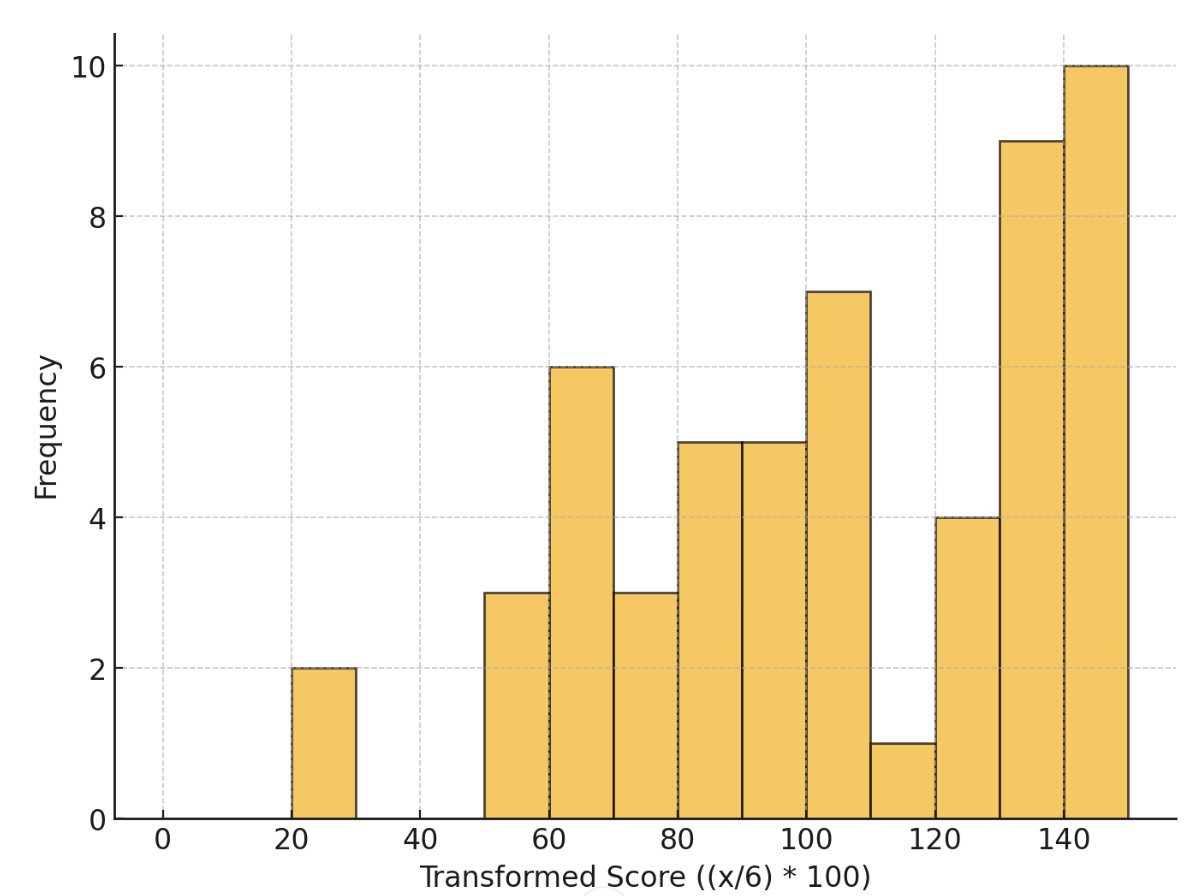
\includegraphics[width=.8\textwidth]{images/problems_quiz_scores}
        \caption{Median Score = 100\%, Mean Score=103.7\%}
\end{figure}
\vfill 

\end{frame}


\begin{frame}{Reading Quiz Scores: Induction}

\begin{figure}[ht]
        \centering
        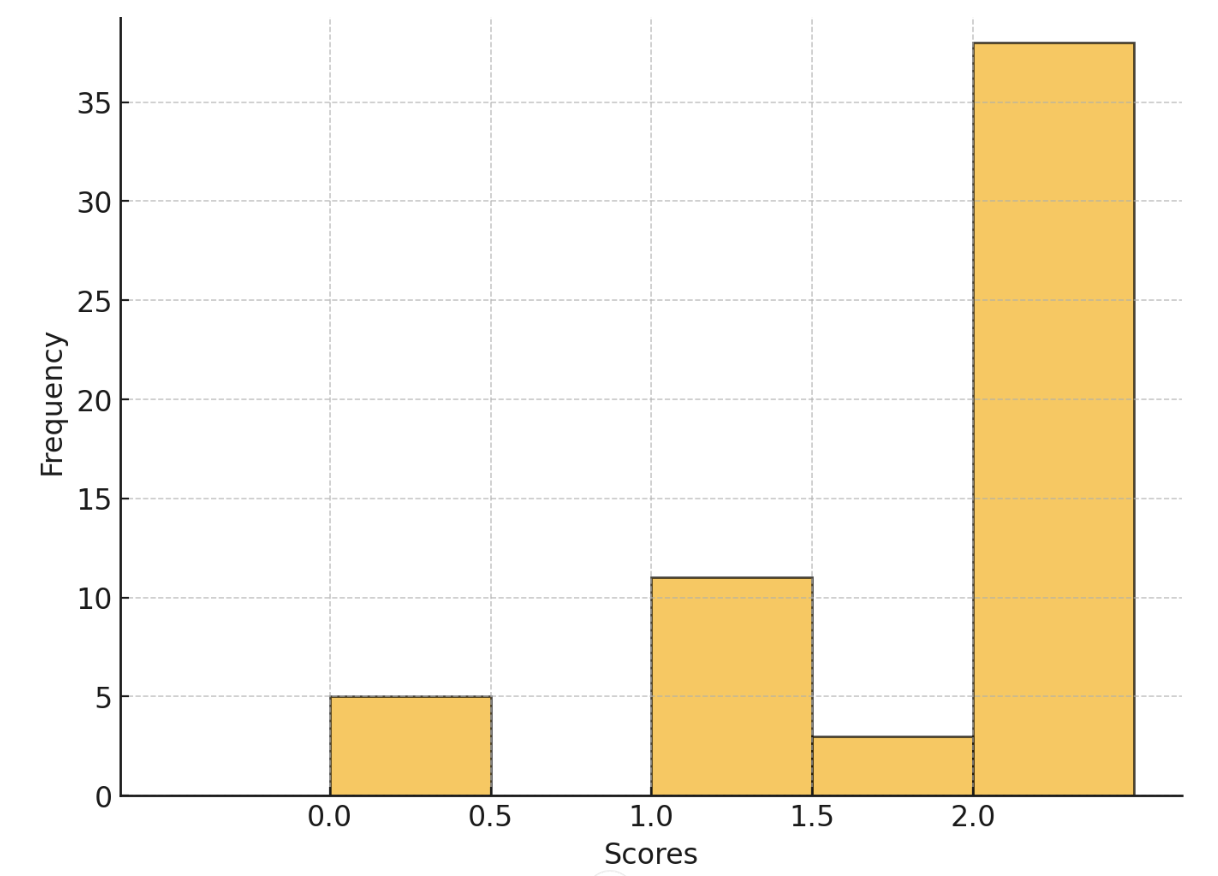
\includegraphics[width=.8\textwidth]{images/reading_quiz_scores}
   		 \caption{Median Score = 2/2 (100\%), Mean Score=1.6/2 (80\%)}
\end{figure}
\vfill 

\end{frame}

\begin{frame}[standout]
Another quick look at the List Group Exercises	
\end{frame}


\begin{frame}[standout]
Some notes on Sets I (Introduction, Subsets) 
\end{frame}




\begin{frame}{Three special sets of numbers}

\begin{mygreenbox}[title=Definition]
The \textbf{integers} are the positive whole numbers, the negative whole numbers, and zero.  That is, the set of integers, denoted by $\mathbb{Z}$ is
\[\mathbb{Z} = \set{\hdots, -3, -2, -1, 0, 1, 2, 3 \hdots}.\] 
\end{mygreenbox}
\vfill 
\begin{mygreenbox}[title=Definition]
The \textbf{natural numbers} (denoted $\mathbb{N}$) are the non-negative integers; that is
\[\mathbb{N} = \set{0, 1, 2, 3 \hdots}.\] 
\end{mygreenbox}
\vfill 
\begin{mygreenbox}[title=Definition]
The \textbf{rational numbers} (denoted $\mathbb{Q}$)  are the numbers formed by dividing two integers a/b, where $b \neq 0$.  That is,
\[\mathbb{Q} = \set{a/b : a,b \in \mathbb{Z}, b \neq 0}.\] 
\end{mygreenbox}
\end{frame}




\begin{frame}{Counting Subsets (Decision Tree Perspective)}

\begin{figure}
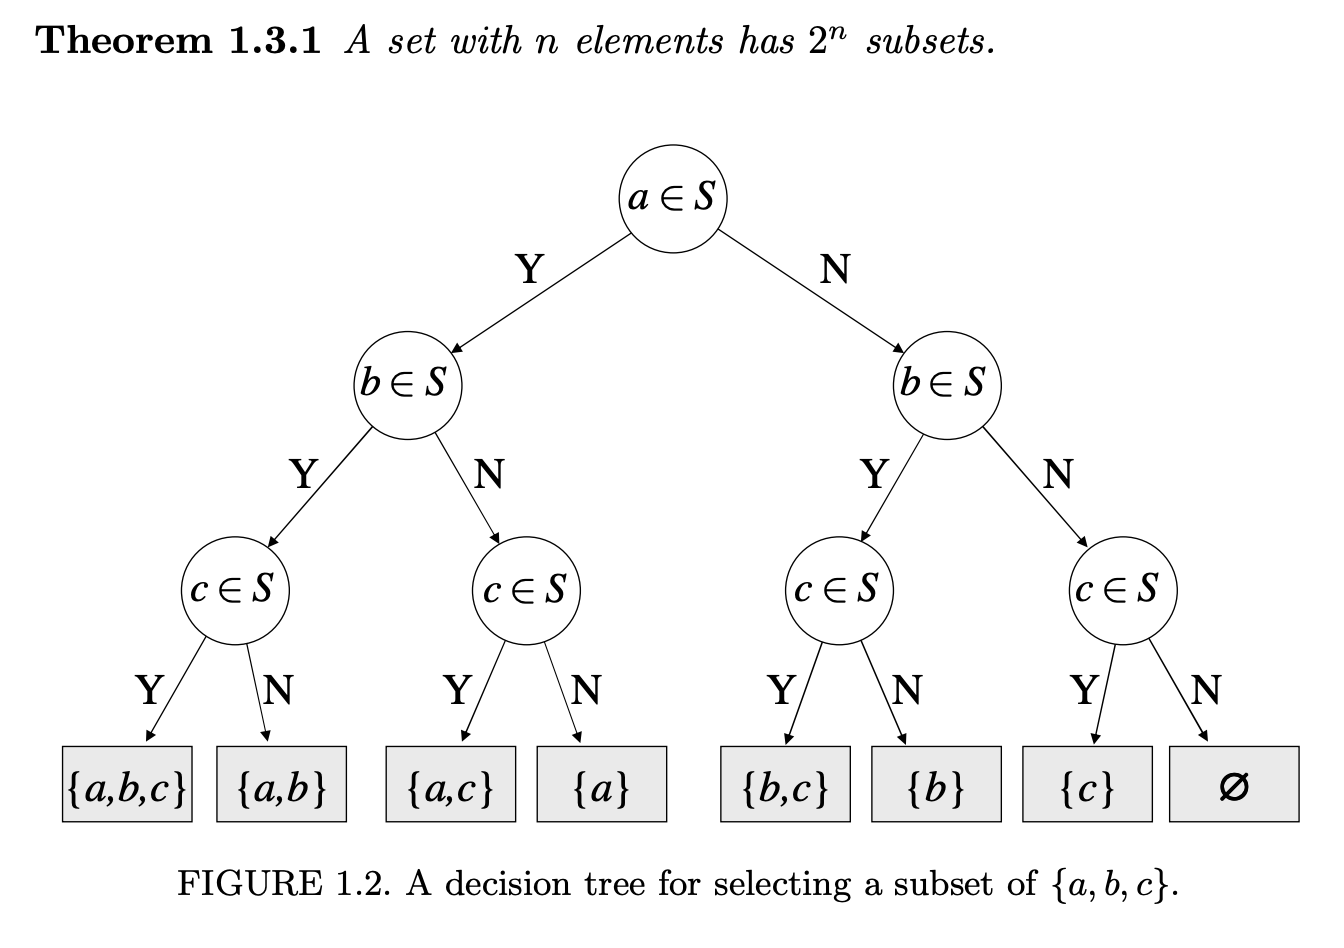
\includegraphics[width=.9\textwidth]{images/decision_tree}

\tiny Source: Lovasz, Pelikan, Vesztergombi. \textit{Discrete Mathematics: Elementary and Beyond.} 	
\end{figure}

\end{frame}

\begin{frame}{Counting Subsets (Enumeration Perspective)}

\begin{figure}
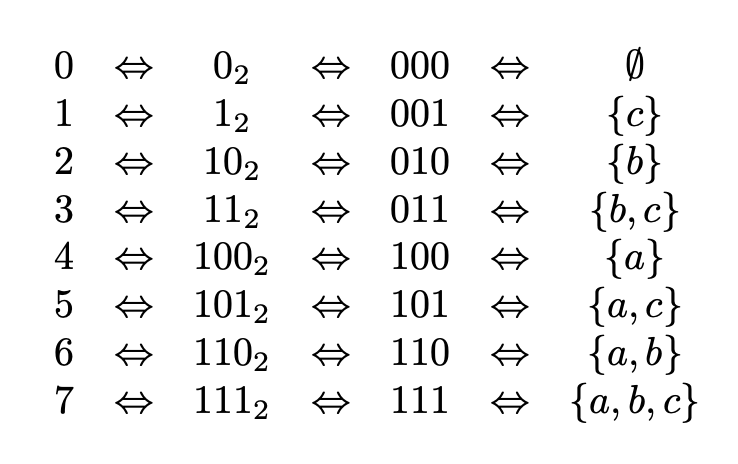
\includegraphics[width=.9\textwidth]{images/correspondence}

\tiny Source: Lovasz, Pelikan, Vesztergombi. \textit{Discrete Mathematics: Elementary and Beyond.} 	
\end{figure}

\vfill \vfill 
\footnotesize 
\textbf{Remark.} Using a code like this, you could determine that the 233rd subset of a 10-element set $\set{a_1, \hdots, a_{10}}$ consists of elements $\set{a_3, a_4, a_5, a_7, a_{10}}$. (That's because 233 in binary is 11101001, which corresponds to the code 0011101001.)
\end{frame}


\begin{frame}{Subtopics from reading}
Scheinerman Sec. 10 (Sets I: Introduction, Subsets) covers the following subtopics
\begin{enumerate}
	\item How to read and write set notation,
	\item How to count the number of subsets of a set,
	\item How to show one set is a subset of the other, and
	\item How to show two sets are equal.
\end{enumerate}

\vfill
Today's group exercises provide additional practice on these subtopics. 
\end{frame}


\begin{frame}
\footnotesize
Group 1: jacob.shepherd1,samuel.hemmen,lucas.jones6\\
Group 2: jonas.zeiler,alexander.goetz,julia.larsen\\
Group 3: james.brubaker,peter.buckley1,alexander.knutson\\
Group 4: joseph.mergenthaler,zeke.baumann,peyton.trigg\\
Group 5: jeremiah.mackey,jack.fry,jacob.ketola\\
Group 6: matthew.nagel,luka.derry,ryan.barrett2\\
Group 7: timothy.true,micaylyn.parker,aaron.loomis\\
Group 8: carsten.brooks,jacob.ruiz1,owen.obrien\\
Group 9: justice.mosso,connor.graville,delaney.rubb\\
Group 10: pendleton.johnston,blake.leone,adam.wyszynski\\
Group 11: bridger.voss,reid.pickert,evan.schoening\\
Group 12: tyler.broesel,carver.wambold,sarah.periolat\\
Group 13: connor.yetter,tristan.nogacki,jakob.kominsky\\
Group 14: griffin.short,emmeri.grooms,kaden.price\\
Group 15: colter.huber,jett.girard,luke.donaldson1\\
Group 16: devon.maurer,evan.barth,anthony.mann\\
Group 17: cameron.wittrock,caitlin.hermanson,connor.mizner\\
Group 18: erik.moore3,yebin.wallace,nolan.scott1\\
Group 19: jada.zorn,michael.oswald,samuel.mosier\\
Group 20: conner.reed1,mason.barnocky,samuel.rollins\\
Group 21: john.fotheringham,derek.price4,william.elder1\\
Group 22: ethan.johnson18,joseph.triem,lynsey.read\\
\end{frame}


\begin{frame}{Group exercises: Sets}


\begin{enumerate}
\item Find the cardinality of the following sets
\begin{itemize}
\item[a)] $\set{x \in \mathbb{Z}: |x| \leq 10}$
\item[b)] $\set{x \in \mathbb{Z}: 1 \leq x^2 \leq 2}$
\item[c)] $\set{x \in \mathbb{Z}: x \in \emptyset}$
\item[d)] $2^{2^{\set{1,2,3}}}$
\item[e)] $\set{x \in 2^{\set{1,2,3,4}}: |x|=1}$
\item[f)] $\set{\set{1,2}, \set{3,4,5}}$
\end{itemize}
\item Let $A= \set{x \in \mathbb{Z}: 4|x}$ and  $B= \set{x \in \mathbb{Z}: 2|x}$.  Prove that $A \subseteq B$.
\item Let $A= \set{0,1,2,3,4}$ and  $B= \set{x \in \mathbb{N}: x^2<17}$.  Prove that $A=B$.
\end{enumerate}

\end{frame}



\begin{frame}{Solution to group exercise \#1 (a-d)}

\small 
\textbf{Solution.}

\begin{itemize}
\item[a)] $\bigg|\set{x \in \mathbb{Z}: |x| \leq 10}\bigg|=\bigg| \set{-10, \hdots, -1, 0, 1, \hdots, 10} \bigg| = 21$
\item[b)] $\bigg|\set{x \in \mathbb{Z}: 1 \leq x^2 \leq 2}\bigg| = \bigg| \set{-1, 1} \bigg| = 2 $
\item[c)] $\bigg| \set{x \in \mathbb{Z}: x \in \emptyset} \bigg| = \bigg| \emptyset \bigg| = 0 $
\item[d)] To find $\bigg|2^{2^{\set{1,2,3}}}\bigg|$, first recall that for any finite set $A$, $2^A$ refers to the set of all subsets of $A$. So setting $A \defeq \set{1,2,3}$, we have 
\[ B \defeq 2^A = 2^{\set{1,2,3}} = \bigg\{ \emptyset, \set{1}, \set{2}, \set{3}, \set{1,2}, \set{1,3}, \set{2,3}, \set{1,2,3} \bigg\}. \]
Now  $2^B$ is the set of all subsets of \textit{that}, 
so
\[2^B = \bigg\{ \emptyset,  \big\{ \set{1}  \big\}, \big\{ \set{2} \big\}, \big\{  \set{3} \big\} , \big\{  \set{1},\set{2} \big\}, \hdots  \big\{  \set{1}, \set{1,2,3}, \set{2}, \set{1,2} \big\} , \hdots \bigg\}  \]
Notably, $B=2^A$ has $2^{|A|} = 2^3=8$ elements, and so $2^B$ has $2^{|B|} = 2^8$ elements. Hence,  $\bigg|2^{2^{\set{1,2,3}}}\bigg| = 2^8$.
\end{itemize}


\end{frame}

\begin{frame}{Solution to group exercise \#1 (e-f)}

\small 
\textbf{Solution.}

\begin{itemize}
\item[e)] To find $\bigg| \set{x \in 2^{\set{1,2,3,4}}: |x|=1} \bigg|$, we proceed similarly as in part (d). The set  $B \defeq 2^{\set{1,2,3,4}}$ refers to the set of all subsets of $\set{1,2,3,4}$.  That is,  
\begin{align*}
 B &= \bigg\{ \emptyset, \set{1}, \set{2}, \set{3}, \set{4}, \set{1,2}, \set{1,3}, \set{1,4}, \set{2,4}, \hdots, \set{1,2,3,4} \bigg\}.	
\end{align*}

In particular $B$ has  $2^{|\set{1,2,3,4}|}=2^4=16$ elements.  Only four of those elements have cardinality 1, namely $\set{1}$, $\set{2}$, $\set{3}$, and $\set{4}$.  Hence $\bigg| \set{x \in 2^{\set{1,2,3,4}}: |x|=1} \bigg| = 4$.
\item[f)] $\bigg| \set{\set{1,2}, \set{3,4,5}} \bigg| = 2$
\end{itemize}


\end{frame}




\begin{frame}{Solution to group exercise \#2}


\textbf{Problem.} Let $A= \set{x \in \mathbb{Z}: 4|x}$ and  $B= \set{x \in \mathbb{Z}: 2|x}$.  Prove that $A \subseteq B$.
\vfill 
\textbf{Solution.} 

\begin{tabularx}{\textwidth}{|L{3cm}|X|}
\hline \textbf{Annotation} & \textbf{Main Text} \\ \hline
 \hlorange{Convert Prop. to ``if-then" form} &  \hlorange{We show that if $x \in A$, then $x \in B$.} \\ \hline
\hlblue{State assumption ("if")} & \hlblue{Let $x \in A$.} \\ \hline
\hlgreen{Unravel defs.} & \hlgreen{Since, $x\in A$, we know that $4|x$.  So by the definition of divisibility, there is some $n \in \mathbb{Z}$ such that $x=4n$.} \\ \hline
\hlred{*** The glue ***} & \hlred{We write $x=4n=2(2n)$} \\ \hline
 \hlgreen{Unravel defs.} & \hlgreen{So there is an integer $c=2n$ such that $x=2c$.  So $2|x$.} \\ \hline
  \hlblue{State conclusion} & \hlblue{Hence, $x \in B$.} \\ \hline
\hline
\end{tabularx}
\end{frame}



\begin{frame}{Solution to group exercise \#3 (Big picture)}


\textbf{Problem.} Let $A= \set{0,1,2,3,4}$ and  $B= \set{x \in \mathbb{N}: x^2<17}$.  Prove that $A=B$.

\vfill 
\textbf{Structure of solution.} To show $A=B$, we show $A \subseteq B$ and $B \subseteq A$.
\begin{itemize}
\item $\boxed{A \subseteq B.}$ We show that if $x \in A $, then $x \in B$.  
\item $\boxed{B \subseteq A.}$	We show that if $x \in B$, then $x \in A$.
\end{itemize}

\end{frame}


\begin{frame}{Solution to group exercise \#3}


\textbf{Problem.} Let $A= \set{0,1,2,3,4}$ and  $B= \set{x \in \mathbb{N}: x^2<17}$.  Prove that $A=B$.

\vfill 
\textbf{Solution.} To show $A=B$, we show $A \subseteq B$ and $B \subseteq A$.
\begin{itemize}
\item $\boxed{A \subseteq B.}$ We show that if $x \in A $, then $x \in B$.  Let $x \in A$.  Then $x \in \set{0,1,2,3,4}$.  Then $x^2 \in \set{0,1,4,9,16}$.  So $x^2<17$.  Hence $x \in B$.
\item $\boxed{B \subseteq A.}$	We show that if $x \in B$, then $x \in A$. Let $x \in B$.  Hence $x \in \mathbb{N}$ and $x^2<17$.  By taking the square root of each side, $x^2<17$ implies   $|x|<\sqrt{17}$.   The only natural numbers satisfying $|x|<\sqrt{17}$ are $0,1,2,3$ and $4$.  Hence $x \in A$. 
\end{itemize}

\end{frame}


\end{document}
